% ============================================================================
\section{Mixture of Experts (MoE)}
% ============================================================================

\begin{frame}[t]{Mixture of Experts (Recap)}
  \begin{itemize}\itemsep0.45em
    \item As covered earlier, an MoE block replaces the single dense feed-forward MLP with several smaller expert MLPs and a router that sends each token to a few of them.
    \item What matters for the 2017-to-2026 comparison is the consequence: total parameters and per-token FLOPs stop being the same number. Capacity can grow while the arithmetic done for each token stays bounded.
    \item This is the flexible-compute item from the roadmap. Sliding windows and MLA make the memory a token costs depend on the architecture; MoE makes the arithmetic it costs depend on the router.
  \end{itemize}
  \vfill
  {\scriptsize Sources: Zhang et al., ``Mixture of Experts in Large Language Models,'' \href{https://arxiv.org/abs/2507.11181}{arXiv:2507.11181}; Kranen \& Nguyen, \href{https://developer.nvidia.com/blog/applying-mixture-of-experts-in-llm-architectures/}{NVIDIA Technical Blog} (Mar.\ 2024).}
\end{frame}

\begin{frame}[t]{MoE milestones}
  \centering
  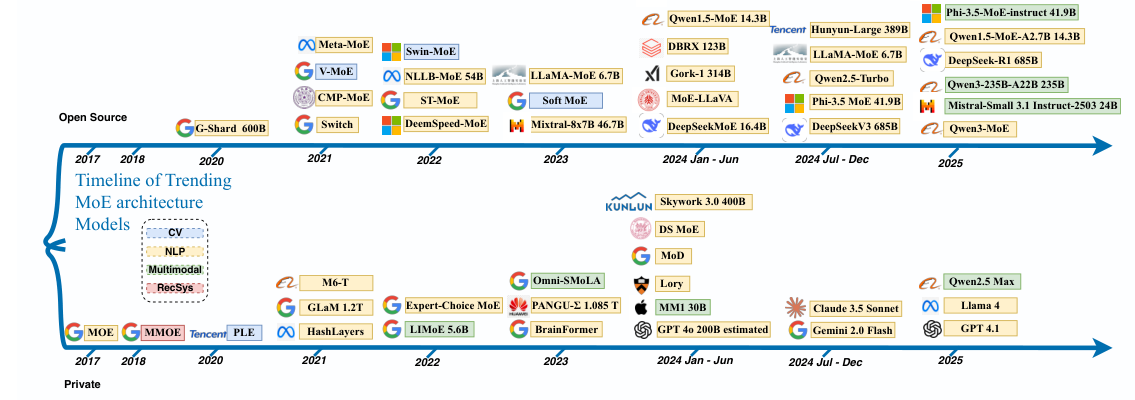
\includegraphics[width=\textwidth,height=0.78\textheight,keepaspectratio]{images/transformers-2017-v-2026/moe_survey_fig1_timeline.png}\\[0.3em]
  {\scriptsize \textit{Reference:} Zhang et al., ``Mixture of Experts in Large Language Models,'' \href{https://arxiv.org/abs/2507.11181}{arXiv:2507.11181}, Figure~1.}
\end{frame}

\begin{frame}[t]{MoE for a decoder-only Transformer}
  \centering
  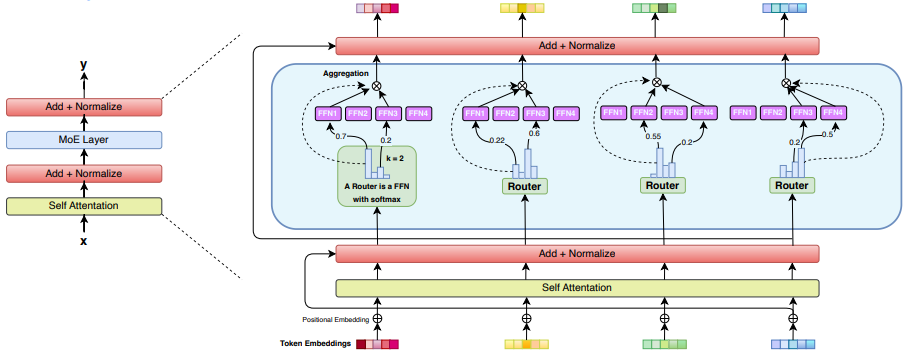
\includegraphics[width=\linewidth,height=0.60\textheight,keepaspectratio]{images/transformers-2017-v-2026/moe_survey_fig3_moe_layer.png}\\[0.2em]
  {\scriptsize Top-$k$ routing with $k=2$ over four expert FFNs, in place of the dense feed-forward sub-block. \textit{Reference:} Zhang et al., \href{https://arxiv.org/abs/2507.11181}{arXiv:2507.11181}, Figure~3.}
\end{frame}

\begin{frame}[t]{Example: Mixtral 8$\times$7B, a common misconception}
  \begin{itemize}
    \item The name invites the arithmetic $8 \times 7\text{B} = 56\text{B}$, and the reading ``eight separate 7B models.'' The released architecture is neither.
    \item Attention layers, norms, and embeddings are shared; only the feed-forward sub-block is replicated eight times. Mixtral 8$\times$7B is 46.7B parameters in total and spends 12.9B on each token, because the router fires only two experts per token.
  \end{itemize}
  \centering
  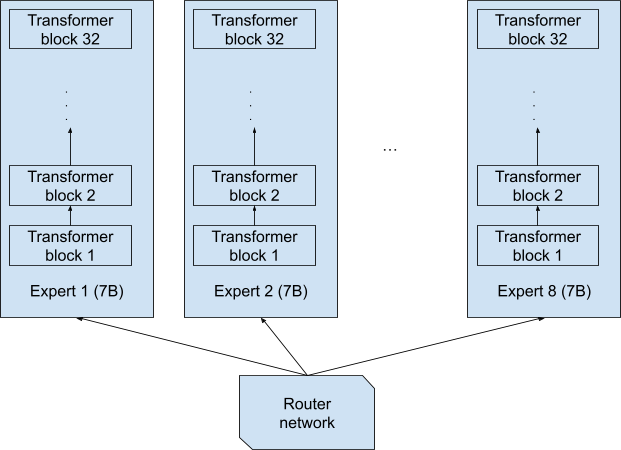
\includegraphics[width=0.68\textwidth,height=0.42\textheight,keepaspectratio]{images/transformers-2017-v-2026/nvidia_blog_mixtral_misread_diagram.png}\\[0.15em]
  {\scriptsize The mental model the name suggests, which is \textit{not} the released design. Kranen \& Nguyen, ``Applying Mixture of Experts in LLM Architectures,'' NVIDIA Technical Blog (2024), \href{https://developer.nvidia.com/blog/applying-mixture-of-experts-in-llm-architectures/}{article}. Parameter counts: Jiang et al., ``Mixtral of Experts,'' \href{https://arxiv.org/abs/2401.04088}{arXiv:2401.04088}.}
\end{frame}

\begin{frame}{MoE: Most Preferred Tokens By Experts}
  \centering
  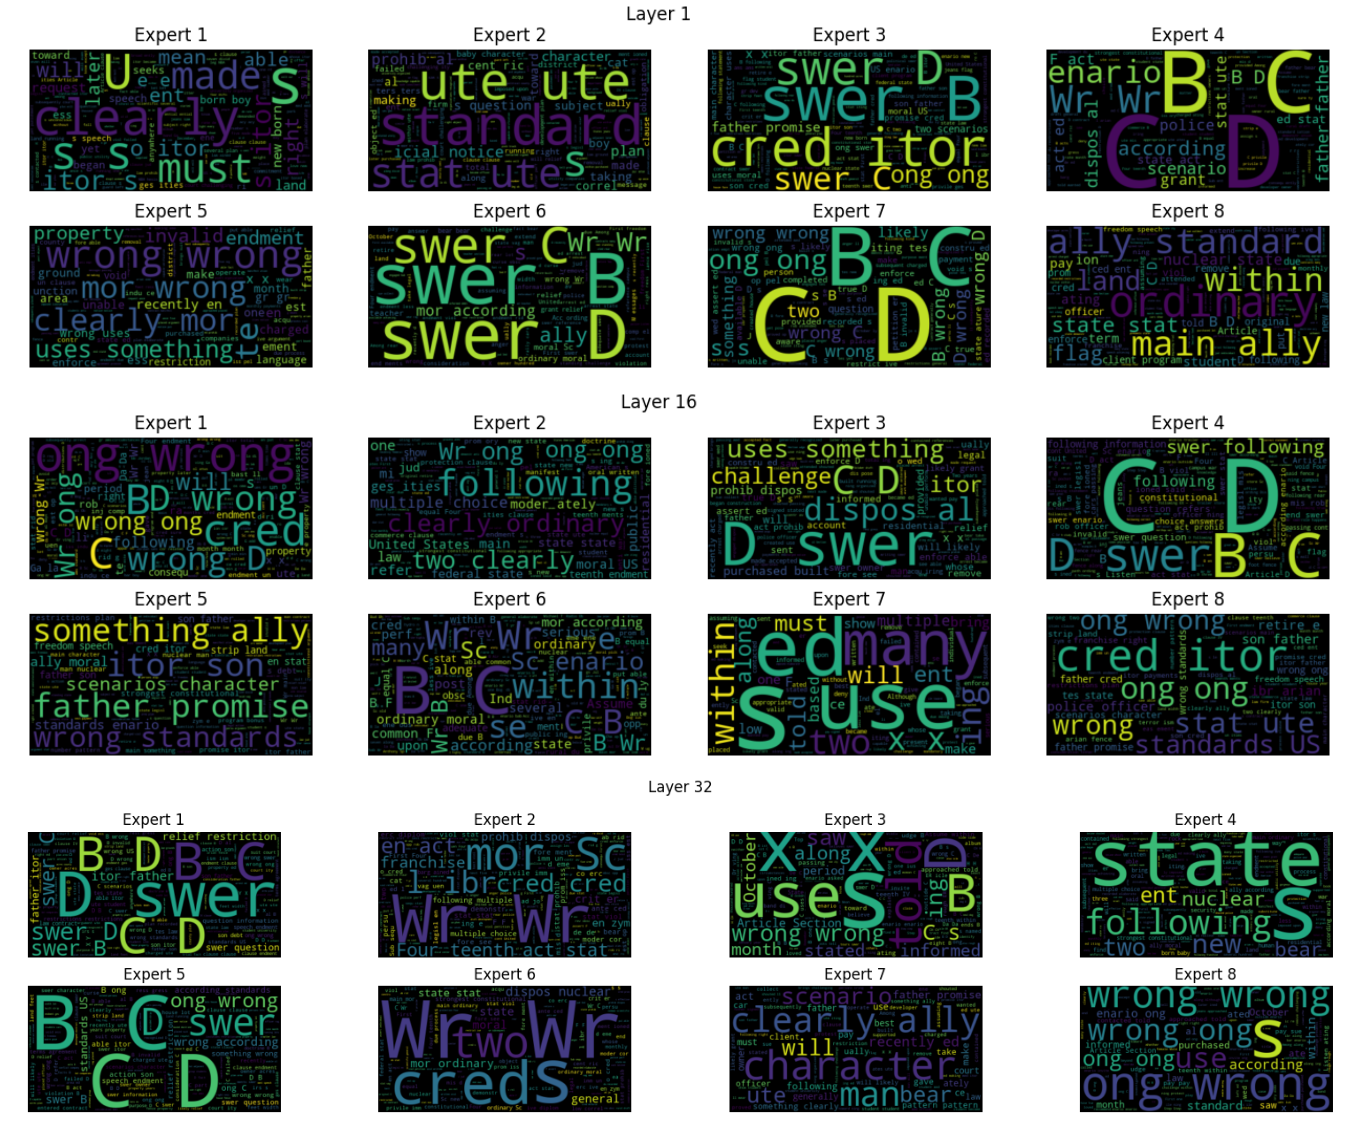
\includegraphics[width=\textwidth,height=0.70\textheight,keepaspectratio]{images/transformers-2017-v-2026/most-common-tokens-processed-moe.png}\\[0.2em]
  {\scriptsize Word clouds of the tokens each Mixtral expert processes most often, at layers 1, 16, and 32. The routing keys on token identity rather than on topic or domain, so ``experts'' are not subject specialists. \textit{Reference:} Kranen \& Nguyen, ``Applying Mixture of Experts in LLM Architectures,'' NVIDIA Technical Blog (2024), \href{https://developer.nvidia.com/blog/applying-mixture-of-experts-in-llm-architectures/}{article}.}
\end{frame}
